\chapter{THỬ NGHIỆM, KẾT QUẢ VÀ THẢO LUẬN}

\section{Thiết lập thí nghiệm}
\begin{itemize}
    \item Chia dữ liệu: 80\% huấn luyện, 20\% kiểm thử, phân tầng theo nhãn, \texttt{random\_state=42}.
    \item Tinh chỉnh siêu tham số: 5-fold CV phân tầng trên tập huấn luyện, tiêu chí F1.
    \item So sánh: 2 luồng đặc trưng $\times$ 3 thuật toán $+$ baseline.
    \item Số dòng huấn luyện và kiểm thử, cùng cấu hình chạy, được ghi trong \texttt{results/run\_info.json}.
\end{itemize}

\section{Kết quả trên tập kiểm thử}
Bảng~\ref{tab:ketqua} tổng hợp kết quả. Bảng được sinh tự động từ \texttt{results/metrics.csv}.
\begin{table}[H]
\centering
\caption{Kết quả các mô hình trên tập kiểm thử}
\label{tab:ketqua}
\resizebox{\textwidth}{!}{\begin{tabular}{llrrrrrrr}
\toprule
Đặc trưng & Mô hình & F1 (CV) & Accuracy & Precision & Recall & F1 & ROC-AUC & PR-AUC \\
\midrule
A\_co\_ban & KNN & 0.600 & 0.790 & 0.618 & 0.543 & 0.578 & 0.829 & 0.605 \\
A\_co\_ban & NaiveBayes & 0.595 & 0.686 & 0.450 & 0.836 & 0.585 & 0.809 & 0.598 \\
A\_co\_ban & DecisionTree & 0.560 & 0.795 & 0.623 & 0.573 & 0.597 & 0.830 & 0.613 \\
A\_co\_ban & Baseline\_LopDaSo & -- & 0.735 & 0.000 & 0.000 & 0.000 & 0.500 & 0.265 \\
B\_cai\_tien & KNN & 0.603 & 0.797 & 0.629 & 0.570 & 0.598 & 0.832 & 0.619 \\
B\_cai\_tien & NaiveBayes & 0.600 & 0.712 & 0.475 & 0.833 & 0.605 & 0.812 & 0.605 \\
B\_cai\_tien & DecisionTree & 0.564 & 0.796 & 0.640 & 0.522 & 0.575 & 0.823 & 0.622 \\
B\_cai\_tien & Baseline\_LopDaSo & -- & 0.735 & 0.000 & 0.000 & 0.000 & 0.500 & 0.265 \\
\bottomrule
\end{tabular}
}
\end{table}

\section{Đường cong và ma trận nhầm lẫn}
\begin{figure}[H]
    \centering
    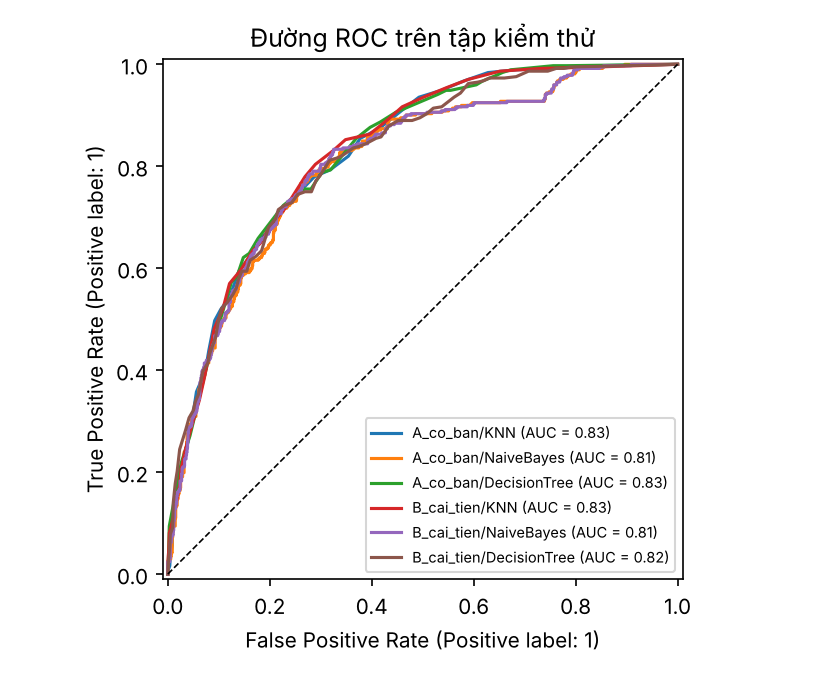
\includegraphics[width=0.6\textwidth]{../results/figures/roc_cac_mo_hinh.png}
    \caption{Đường ROC của các mô hình trên tập kiểm thử}
    \label{fig:roc}
    \Nguon{Nhóm tự vẽ từ kết quả thí nghiệm}
\end{figure}

\begin{figure}[H]
    \centering
    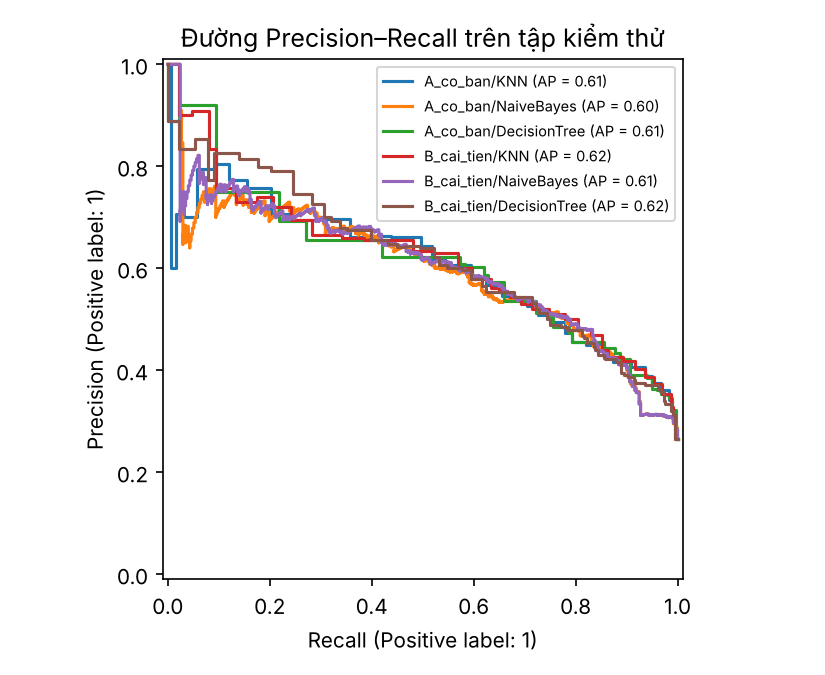
\includegraphics[width=0.6\textwidth]{../results/figures/pr_cac_mo_hinh.png}
    \caption{Đường Precision--Recall của các mô hình trên tập kiểm thử}
    \label{fig:pr}
    \Nguon{Nhóm tự vẽ từ kết quả thí nghiệm}
\end{figure}

\begin{figure}[H]
    \centering
    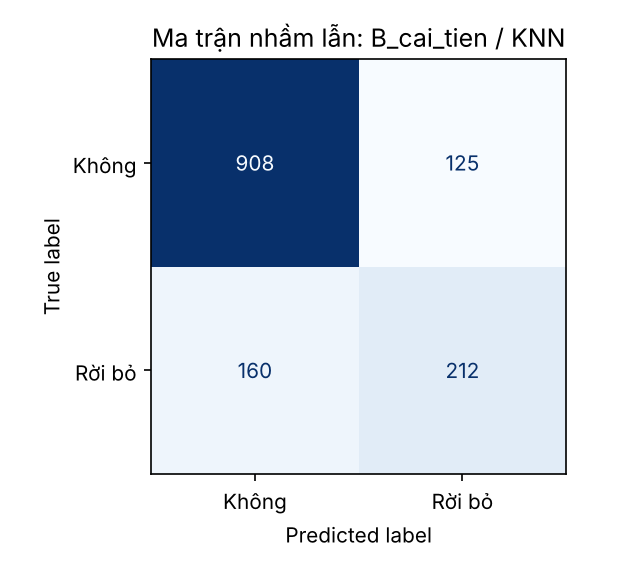
\includegraphics[width=0.45\textwidth]{../results/figures/cm_best.png}
    \caption{Ma trận nhầm lẫn của cấu hình được chọn}
    \label{fig:cm}
    \Nguon{Nhóm tự vẽ từ kết quả thí nghiệm}
\end{figure}

\section{Phân tích lỗi}
Bảng lỗi theo nhóm được lưu tại \texttt{results/error\_by\_group.csv}, và danh sách các khách hàng rời bỏ bị bỏ sót
(FN với xác suất rời bỏ thấp nhất) tại \texttt{results/false\_negative\_examples.csv}. Nhóm phân tích các nhóm có tỷ lệ sai cao,
số FN và FP, rồi đối chiếu với giả thuyết đã nêu ở chương 1 và đặc trưng ở chương 2.

\section{Thảo luận}
\subsection{So sánh với mốc baseline}
Mô hình mốc luôn dự đoán ``không rời bỏ'' đạt Accuracy 73,5\%, nhưng Recall và F1 đều bằng 0 và không phát hiện được khách hàng nào sắp rời bỏ.
Mọi mô hình học máy đều vượt mốc này rõ rệt về Recall, F1 và ROC-AUC (0,81--0,83 so với 0,50). Accuracy không phản ánh được điều này, nên nhóm không dùng Accuracy làm tiêu chí chính.

\subsection{Chọn mô hình và so sánh hai luồng đặc trưng}
Theo quy tắc đã nêu ở chương 2, cấu hình được chọn là \textbf{KNN với luồng B} (F1 trung bình CV 0,603; F1 trên tập kiểm thử 0,598; Recall 0,570; Precision 0,629; ROC-AUC 0,832).
Tuy nhiên, khoảng cách giữa các cấu hình hàng đầu trong CV rất nhỏ: KNN luồng B 0,603, Naive Bayes luồng B 0,600 và KNN luồng A 0,600.
Trên tập kiểm thử, Naive Bayes luồng B có F1 cao nhất (0,605), còn Cây quyết định luồng B có PR-AUC cao nhất (0,622). Vì vậy, \textbf{không có một mô hình vượt trội rõ ràng}; các mô hình khác nhau ở cách đánh đổi giữa Precision và Recall.

Đặc trưng kỹ thuật của luồng B cải thiện KNN (F1 từ 0,578 lên 0,598) và Naive Bayes (từ 0,585 lên 0,605), nhưng làm giảm F1 của Cây quyết định (từ 0,597 xuống 0,575).
Với một lần chia dữ liệu và độ chênh lệch nhỏ, nhóm chưa thể khẳng định luồng B tốt hơn; cần kiểm định lặp lại nhiều lần để có kết luận chắc chắn.

\subsection{Cách đánh đổi giữa Precision và Recall}
Naive Bayes có Recall cao nhất (0,833) nhưng Precision thấp (0,475), tức là phát hiện được gần hết khách hàng rời bỏ nhưng phải chăm sóc nhiều khách không có nguy cơ.
Cây quyết định và KNN thiên về Precision cao hơn (0,62--0,64) nhưng bỏ sót nhiều khách rời bỏ hơn. Lựa chọn ngưỡng quyết định phụ thuộc vào chi phí chăm sóc và chi phí mất khách; nhóm giữ ngưỡng mặc định 0,5 và không tinh chỉnh ngưỡng trên tập kiểm thử để tránh rò rỉ.

\subsection{Đặc trưng quan trọng}
Biểu đồ độ quan trọng của cây quyết định (luồng B, Bảng trong \texttt{results/dt\_feature\_importance\_top15.csv}) cho thấy:
hợp đồng theo tháng chiếm 46,6\% tổng độ quan trọng, tiếp theo là \texttt{tenure} (16,0\%), dịch vụ cáp quang (14,5\%), \texttt{TotalCharges} (5,9\%) và \texttt{MonthlyCharges} (4,5\%).
Đặc trưng kỹ thuật \texttt{charge\_per\_tenure} đứng thứ sáu với 2,8\%, cho thấy đặc trưng này có đóng góp nhưng không phải yếu tố chính.
Kết quả này phù hợp với nghiệp vụ: khách hàng hợp đồng ngắn hạn, mới gắn bó và dùng cáp quang có nhiều khả năng rời bỏ.

\subsection{Phân tích lỗi}
Phân tích trên mô hình KNN luồng B (\texttt{results/error\_by\_group.csv}) cho các nhận xét sau:
\begin{itemize}
    \item \textbf{Hợp đồng theo tháng} có tỷ lệ sai cao nhất (31,2\%): 118 khách rời bỏ bị bỏ sót (FN) và 124 khách không rời bỏ bị cảnh báo nhầm (FP). Hợp đồng hai năm chỉ sai 2,4\%.
    \item \textbf{Cáp quang} có tỷ lệ sai 25,1\%, và chủ yếu là FP (98 so với 58 FN). Mô hình có xu hướng dự đoán rời bỏ quá mức ở nhóm này, phù hợp với việc nhóm này có tỷ lệ rời bỏ thực tế cao (41,9\%) nhưng đa số vẫn ở lại.
    \item \textbf{Thời gian gắn bó 0--12 tháng} có tỷ lệ sai 33,3\%, cao nhất trong các nhóm thời gian. Nhóm này vừa khó dự đoán vừa có tỷ lệ rời bỏ thực tế cao (47,4\%).
    \item Các ca bỏ sót (\texttt{false\_negative\_examples.csv}) thường là khách hợp đồng một năm hoặc hai năm, có xác suất rời bỏ dự đoán gần 0. Những trường hợp này không thể hiện qua các đặc trưng hiện có, có thể do lý do ngoài dữ liệu như chất lượng dịch vụ hoặc cạnh tranh.
\end{itemize}

\section{Hạn chế}
\begin{itemize}
    \item \textbf{Kết quả nằm sát biên lưới tham số.} KNN chọn $k=41$ (giá trị lớn nhất trong lưới), Naive Bayes luồng B chọn $\text{var\_smoothing}=10^{-9}$ (giá trị nhỏ nhất), Cây quyết định chọn \texttt{min\_samples\_leaf}=50 (giá trị lớn nhất). Cấu hình tốt hơn có thể nằm ngoài lưới đã thử.
    \item \textbf{Một lần chia train/test.} Chênh lệch giữa các mô hình rất nhỏ nên thứ hạng có thể thay đổi với cách chia khác. Hướng khắc phục là lặp lại đánh giá với nhiều hạt giống ngẫu nhiên hoặc dùng kiểm định thống kê.
    \item Dữ liệu là ảnh chụp tại một thời điểm, không có chuỗi thời gian theo tháng, nên không mô hình hóa được xu hướng thay đổi hành vi.
    \item Chưa so sánh với hồi quy logistic hay mô hình ensemble vì không thuộc danh sách thuật toán của học phần; đây là phần mở rộng hợp lý.
\end{itemize}
